% !TEX root = ../main.tex
% File: chapters_part1/chap5_5.tex
% Nội dung cho Chương 5, Phần 5

\section{Các phương pháp Căn chỉnh (Alignment) với Con người}
\label{sec:alignment_methods}

Sau khi đã qua bước Tinh chỉnh theo chỉ dẫn (Instruction Tuning), mô hình của chúng ta đã học được cách tuân theo mệnh lệnh. Tuy nhiên, nó vẫn có thể tạo ra các kết quả không mong muốn:
\begin{itemize}
    \item \textbf{Không hữu ích (Unhelpful):} Trả lời "Tôi không biết" quá thường xuyên, hoặc đưa ra các câu trả lời không liên quan.
    \item \textbf{Không trung thực (Dishonest) / Bịa đặt (Hallucination):} Tự tin bịa đặt thông tin, trích dẫn các nguồn không tồn tại.
    \item \textbf{Độc hại (Harmful):} Tạo ra các nội dung nguy hiểm, thiên vị, hoặc xúc phạm, ngay cả khi không được yêu cầu trực tiếp.
\end{itemize}

Vấn đề là, các khái niệm như "hữu ích", "trung thực", "vô hại" rất phức tạp, mơ hồ và phụ thuộc vào ngữ cảnh. Chúng ta không thể định nghĩa chúng bằng một hàm mất mát đơn giản. Chúng ta cần một cách để truyền đạt những sở thích (preferences) tinh tế của con người vào mô hình. Đây là lúc các phương pháp \textbf{Căn chỉnh (Alignment)} phát huy tác dụng.

\subsection{Mục tiêu Căn chỉnh: Bộ ba H (The 3 H's)}
\label{ssec:alignment_goals}
Mục tiêu cuối cùng của quá trình căn chỉnh thường được tóm gọn trong bộ ba nguyên tắc, được đề xuất bởi các nhà nghiên cứu tại Anthropic, thường được gọi là "HHH":
\begin{enumerate}
    \item \textbf{Helpful (Hữu ích):} Mô hình nên cố gắng thực hiện ý định của người dùng một cách hiệu quả và đầy đủ. Nó nên tuân theo chỉ dẫn, thay vì lảng tránh hoặc từ chối một cách không cần thiết.
    \item \textbf{Honest (Trung thực):} Mô hình không nên cố ý lừa dối hoặc bịa đặt thông tin. Khi không chắc chắn, nó nên thể hiện sự không chắc chắn đó thay vì đưa ra một câu trả lời sai một cách tự tin.
    \item \textbf{Harmless (Vô hại):} Mô hình không nên gây ra tác hại, dù là cho người dùng trực tiếp hay cho xã hội nói chung. Nó phải từ chối các yêu cầu tạo ra nội dung nguy hiểm, phi đạo đức, hoặc bất hợp pháp.
\end{enumerate}
Việc cân bằng ba mục tiêu này là một thách thức lớn (ví dụ, một câu trả lời hoàn toàn trung thực có thể gây tổn thương và không "vô hại"). Các phương pháp căn chỉnh dưới đây là nỗ lực để đạt được sự cân bằng này.

\subsection{Học Tăng cường từ Phản hồi Con người (RLHF)}
\label{ssec:rlhf}
Reinforcement Learning from Human Feedback (RLHF) \cite{christiano2017deep, stiennon2020learning} là phương pháp tiên phong và nổi tiếng nhất để căn chỉnh LLM, là công nghệ cốt lõi đằng sau thành công của ChatGPT. Đây là một quy trình gồm ba bước phức tạp.

\begin{center}
    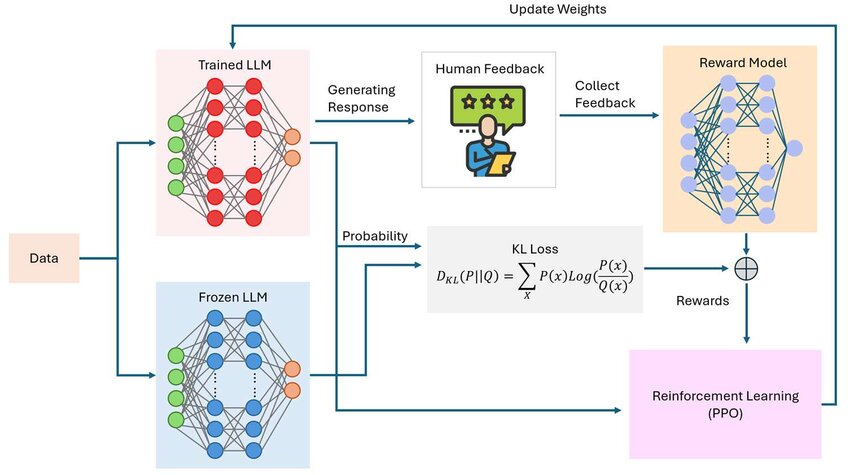
\includegraphics[width=1.0\textwidth]{rlhf_pipeline.png}
    \captionof{figure}{Quy trình ba bước của RLHF: (1) Tinh chỉnh có giám sát (SFT), (2) Huấn luyện Mô hình Phần thưởng (RM), (3) Tối ưu hóa bằng Học tăng cường (PPO).}
    \label{fig:rlhf_pipeline}
\end{center}

\subsubsection{Bước 1: Tinh chỉnh có giám sát (Supervised Fine-Tuning - SFT)}
\begin{itemize}
    \item \textbf{Mục tiêu:} Dạy cho mô hình văn phong và định dạng của một trợ lý đối thoại.
    \item \textbf{Quy trình:} Đây chính là bước \textbf{Instruction Tuning} mà chúng ta đã học ở mục \ref{sec:instruction_tuning}. Một nhóm nhỏ những người gán nhãn chuyên nghiệp (labelers) sẽ viết các prompt chất lượng cao và các câu trả lời mẫu lý tưởng. Mô hình ngôn ngữ cơ sở (base LLM) sau đó được fine-tune trên bộ dữ liệu này.
    \item \textbf{Kết quả:} Một mô hình SFT có khả năng tuân theo chỉ dẫn, nhưng chưa được căn chỉnh sâu về các sở thích tinh tế.
\end{itemize}

\subsubsection{Bước 2: Huấn luyện một Mô hình Phần thưởng (Reward Model - RM)}
Đây là bước cốt lõi của RLHF.
\begin{itemize}
    \item \textbf{Mục tiêu:} Dạy cho một mô hình khác (gọi là Mô hình Phần thưởng) cách \textbf{đánh giá chất lượng} của một câu trả lời, mô phỏng lại sở thích của con người. RM sẽ nhận vào một cặp (prompt, response) và trả về một điểm số duy nhất thể hiện mức độ "tốt" của câu trả lời đó.
    \item \textbf{Quy trình thu thập dữ liệu:}
        \begin{enumerate}
            \item Lấy một prompt từ bộ dữ liệu.
            \item Cho mô hình SFT (từ bước 1) sinh ra nhiều câu trả lời khác nhau (ví dụ: 4 đến 9 câu).
            \item Yêu cầu người gán nhãn \textbf{xếp hạng (rank)} các câu trả lời này từ tốt nhất đến tệ nhất, dựa trên các tiêu chí HHH.
        \end{enumerate}
        Việc yêu cầu con người xếp hạng thay vì cho điểm trực tiếp sẽ dễ dàng và nhất quán hơn nhiều.
    \item \textbf{Quy trình huấn luyện RM:}
        \begin{itemize}
            \item Dữ liệu huấn luyện của RM là các cặp so sánh. Ví dụ, với một prompt, nếu câu trả lời $A$ được xếp hạng cao hơn câu trả lời $B$, chúng ta có một điểm dữ liệu `(prompt, response\_A, response\_B)` với nhãn `A > B`.
            \item RM (thường là một mô hình Encoder-Only như RoBERTa hoặc một LLM đã được loại bỏ lớp cuối) được huấn luyện để dự đoán xác suất một câu trả lời sẽ được con người ưa thích hơn. Cụ thể, nó được huấn luyện để gán một điểm số $r(x, y)$ cho mỗi cặp (prompt $x$, response $y$) sao cho với các cặp được xếp hạng, $r(x, y_{\text{thích hơn}}) > r(x, y_{\text{kém hơn}})$.
        \end{itemize}
    \item \textbf{Kết quả:} Một Mô hình Phần thưởng có khả năng "chấm điểm" bất kỳ câu trả lời nào, hoạt động như một "giám khảo AI" được đào tạo từ sở thích của con người.
\end{itemize}

\subsubsection{Bước 3: Tối ưu hóa bằng Học tăng cường (Reinforcement Learning)}
\begin{itemize}
    \item \textbf{Mục tiêu:} Sử dụng Mô hình Phần thưởng để tinh chỉnh chính sách của mô hình SFT.
    \item \textbf{Thiết lập Học tăng cường (RL):}
        \begin{itemize}
            \item \textbf{Tác tử (Agent):} Chính là mô hình SFT.
            \item \textbf{Chính sách (Policy):} Là chính mô hình SFT, quyết định xác suất sinh ra một token khi biết trạng thái.
            \item \textbf{Không gian hành động (Action Space):} Toàn bộ từ vựng của mô hình.
            \item \textbf{Môi trường (Environment):} Người dùng đưa ra một prompt.
            \item \textbf{Phần thưởng (Reward):} Điểm số được tính bởi \textbf{Mô hình Phần thưởng} (từ bước 2).
        \end{itemize}
    \item \textbf{Quy trình huấn luyện:}
        \begin{enumerate}
            \item Lấy một prompt từ bộ dữ liệu.
            \item Mô hình SFT (chính sách hiện tại) sinh ra một câu trả lời.
            \item Mô hình Phần thưởng chấm điểm câu trả lời này để tạo ra một phần thưởng.
            \item Phần thưởng này được sử dụng làm tín hiệu để cập nhật các trọng số của mô hình SFT thông qua một thuật toán tối ưu hóa chính sách như \textbf{Proximal Policy Optimization (PPO) \cite{schulman2017proximal}}.
            \item Một thành phần quan trọng được thêm vào hàm phần thưởng là một \textbf{hình phạt KL-divergence}. Nó đo lường sự khác biệt giữa chính sách hiện tại và chính sách của mô hình SFT gốc. Hình phạt này ngăn không cho mô hình "tối ưu quá mức" cho Mô hình Phần thưởng và đi quá xa so với những gì nó đã học, giúp nó không bị "quên" các kiến thức ngôn ngữ cơ bản.
        \end{enumerate}
    \item \textbf{Kết quả:} Một mô hình đã được căn chỉnh cuối cùng, có khả năng sinh ra các câu trả lời vừa tuân theo chỉ dẫn, vừa được con người ưa thích.
\end{itemize}

\subsection{Các phương pháp thay thế: Hướng tới sự Đơn giản và Ổn định}
\label{ssec:rlhf_alternatives}
RLHF cực kỳ mạnh mẽ nhưng cũng rất phức tạp, tốn kém và không ổn định để huấn luyện. Điều này đã thúc đẩy việc tìm kiếm các phương pháp thay thế đơn giản hơn.

\subsubsection{Direct Preference Optimization (DPO)}
\begin{itemize}
    \item \textbf{Ý tưởng cốt lõi (Rafailov et al., 2023) \cite{rafailov2023direct}:} Tại sao phải huấn luyện một Mô hình Phần thưởng riêng biệt rồi lại dùng RL để tối ưu hóa nó? Chúng ta có thể tối ưu hóa trực tiếp trên dữ liệu sở thích của con người chỉ bằng một hàm mất mát duy nhất.
    \item \textbf{Cơ chế:} DPO chứng minh rằng hàm mất mát của RLHF có thể được viết lại thành một hàm mất mát đơn giản, có thể được tối ưu hóa trực tiếp bằng cách fine-tuning có giám sát.
    \item \textbf{Quy trình:} DPO chỉ cần dữ liệu so sánh (prompt, câu trả lời được thích hơn, câu trả lời kém hơn) và fine-tune mô hình SFT trực tiếp trên dữ liệu này. Nó tối ưu hóa mô hình để tăng xác suất của các câu trả lời được ưa thích và giảm xác suất của các câu trả lời không được ưa thích, trong khi vẫn duy trì một khoảng cách nhất định với mô hình tham chiếu.
    \item \textbf{Lợi ích:} Đơn giản hơn rất nhiều, ổn định hơn, và thường cho kết quả tương đương hoặc tốt hơn RLHF. DPO đang nhanh chóng trở thành một tiêu chuẩn mới cho việc căn chỉnh.
\end{itemize}

\subsubsection{Constitutional AI (CAI)}
\begin{itemize}
    \item \textbf{Ý tưởng cốt lõi (Bai et al., 2022) \cite{bai2022constitutional}:} Giảm sự phụ thuộc vào phản hồi của con người, đặc biệt là trong việc làm cho mô hình trở nên vô hại. Thay vì yêu cầu con người gán nhãn các nội dung độc hại, hãy để mô hình tự học cách tuân theo một bộ \textbf{"hiến pháp" (constitution)} gồm các nguyên tắc cơ bản.
    \item \textbf{Quy trình (Giai đoạn RL from AI Feedback - RLAIF):}
        \begin{enumerate}
            \item \textbf{Phê bình (Critique):} Cho mô hình SFT xem một prompt có thể gây hại. Yêu cầu chính mô hình (hoặc một mô hình khác) phê bình câu trả lời của nó dựa trên các nguyên tắc trong hiến pháp.
            \item \textbf{Sửa đổi (Revision):} Yêu cầu mô hình viết lại câu trả lời dựa trên những lời phê bình đó để làm cho nó tuân thủ hiến pháp hơn.
            \item \textbf{Huấn luyện:} Cặp (câu trả lời gốc, câu trả lời đã sửa đổi) bây giờ có thể được sử dụng làm dữ liệu sở thích (sửa đổi > gốc) để huấn luyện một Mô hình Phần thưởng hoặc sử dụng DPO.
        \end{enumerate}
    \item \textbf{Lợi ích:} Tự động hóa quá trình tạo dữ liệu căn chỉnh về tính vô hại, giảm bớt gánh nặng và sự phơi nhiễm của con người với các nội dung độc hại.
\end{itemize}

Quá trình căn chỉnh là bước cuối cùng và cũng là một trong những bước phức tạp nhất, biến một công cụ mạnh mẽ thành một đối tác đáng tin cậy.

\bigskip
\hrule
\bigskip

\begin{center}
    \textbf{\Large KẾT THÚC CHƯƠNG 5}
\end{center}

\textit{Chương này đã trang bị cho bạn những kỹ thuật thiết yếu để biến một mô hình nền tảng thô thành một công cụ hữu ích và an toàn. Chúng ta đã đi từ các phương pháp tinh chỉnh kinh điển, đến các kỹ thuật PEFT hiệu quả, và khám phá sức mạnh của việc "trò chuyện" với mô hình thông qua Prompt Engineering. Cuối cùng, chúng ta đã tìm hiểu các quy trình phức tạp như RLHF và DPO để căn chỉnh hành vi của mô hình với sở thích của con người. Với một mô hình đã được tinh chỉnh và căn chỉnh, chúng ta đã có một "bộ não" AI mạnh mẽ. Tuy nhiên, để giải quyết các vấn đề phức tạp trong thế giới thực, bộ não này cần có khả năng truy cập kiến thức bên ngoài, sử dụng công cụ, và thậm chí tương tác với các phương thức khác như hình ảnh. Chương tiếp theo sẽ khám phá các hệ thống và kiến trúc nâng cao kết hợp LLM với các thành phần bên ngoài, tạo ra các ứng dụng AI thực sự toàn diện.}